\chapter{Fonctions affines}\label{ChFonctionsAffines}

\begin{acquis}
\begin{itemize}
\item Savoir reconnaître une fonction affine et/ou l’utiliser dans un problème;
\item Savoir tracer le graphe d’une fonction affine;
\item Savoir calculer la pente d’une fonction affine à l’aide de deux points;
\item Savoir déterminer le zéro d’une fonction affine;
\item Savoir déterminer l’expression algébrique d’une fonction affine à partir de son graphe;
\item Savoir déterminer le sens de variation d’une fonction affine;
\item Savoir déterminer le signe d’une fonction affine à l’aide d’un tableau de signe (graphiquement et algébriquement).
\end{itemize}
\end{acquis}

\exercicesbase
\begin{colonne*exercice}

\serie{Fonctions affines}

\begin{exercice}
On considère les fonctions suivantes définies sur $\mathbb{R}$, préciser à chaque fois en justifiant si la fonction est une fonction affine? linéaire?
\begin{enumerate}
\item $f(x)=3x-6$
\item $g(x)=\sqrt{5}x$
\item $u(x)=3(x-1)+3$
\item $v(x)=(x+1)^2-(x^2-1)$
\end{enumerate}
\end{exercice}

\begin{exercice}
Soit $f$ une fonction affine définie, pour tout nombre réel, par $f(x)=-3x+2$.
\begin{enumerate}
\item Déterminer $f(0)$ et $f(-1)$;
\item Calculer l'image de $\dfrac{1}{3}$ par $f$;
\item Résoudre $f(x)=-5$;
\item Calculer la préimage de 4 par $f$.
\end{enumerate}
\end{exercice}

\begin{exercice}
On appelle $x$ le nombre de litres de carburant pris à la pompe et $y$ le prix payé. Le litre de carburant coûte $1,32$ CHF.
\begin{enumerate}
\item Ecrire $y$ en fonction de $x$. La relation liant $x$ et $y$ est-elle une fonction linéaire? Si oui, quel est son coefficient?
\item Compléter le tableau suivant :
\end{enumerate}
\renewcommand{\arraystretch}{2}
\begin{tabular}{|p{1.2cm}|p{0.8cm}|p{0.8cm}|p{0.8cm}|p{0.8cm}|p{0.8cm}|}
 \hline
quantité (en $L$)&$30$&$20$&$50$&35&\\\hline
prix (en CHF)& &&&&$52,8$\\\hline
 \end{tabular}
\end{exercice}

\begin{exercice}
Dans chacun des cas suivants, $f$ est une fonction linéaire. Compléter les tableaux suivants : \\
\begin{tabular}{c}
\renewcommand{\arraystretch}{2}
1. \begin{tabular}{|p{2cm}|p{1.2cm}|p{1.1cm}|}
 \hline
$x$&$\dfrac{3}{4}$&$-\dfrac{5}{6}$\\\hline
$f(x)$&&$-\dfrac{1}{2}$\\\hline
 \end{tabular}\\\\
\renewcommand{\arraystretch}{2}
2. \begin{tabular}{|p{2cm}|p{1.2cm}|p{1.1cm}|}
 \hline
$x$&&$-\dfrac{4}{15}$\\\hline
$f(x)$&$-\dfrac{5}{3}$&$0,4$\\\hline
 \end{tabular}\\\\
\renewcommand{\arraystretch}{2}
3. \begin{tabular}{|p{2cm}|p{1.2cm}|p{1.1cm}|}
 \hline
$x$&$-\dfrac{7}{5}$&$-\dfrac{6}{7}$\\\hline
$f(x)$&&$-10$\\\hline
 \end{tabular}\\\\
\renewcommand{\arraystretch}{2}
4. \begin{tabular}{|p{2cm}|p{1.2cm}|p{1.1cm}|}
 \hline
$x$&$-1$&$-\frac{1}{3}$\\\hline
$f(x)$&&$-2$\\\hline
 \end{tabular}\\
\end{tabular}
\end{exercice}

\begin{exercice}
Les deux parties sont indépendantes.\\
\begin{enumerate}
\item Un objet coûte 20 CHF. Combien coûtera-t-il après une hausse de 20\%?
\item Après une baisse de 10\%, un objet coûte 22,50 CHF. Quel était son prix avant la baisse?
\end{enumerate}
\end{exercice}

\begin{exercice}
On considère les fonctions suivantes définies sur $\mathbb{R}$:\\\\
\begin{tabular}{p{4cm}p{4cm}}
\textbf{a)} $f(x)=3x$   &   \textbf{b)} $g(x)=-2x$    \\\\
\textbf{c)} $u(x)=\displaystyle\frac{2}{3}x$    &  \textbf{d)} $v(x)=\displaystyle-\frac{3}{7}x$    \\\\
\end{tabular} 
\begin{enumerate}
\item Représenter graphiquement chacune de ces fonctions
\item Représenter graphiquement les points suivants $A\left( 1;\frac{2}{3}\right) $, $B(6;4)$, $C(1;0)$ et $D(3;1)$.
\item Ces points appartiennent-ils à une des droites représentant les fonctions linéaires ci-dessus? Justifier votre réponse par un calcul.
\end{enumerate}
\end{exercice}

\begin{exercice}
Soit $f$ une fonction définie sur $\mathbb{R}$ par $f(x)=-\dfrac{3}{2}x-5$. Les points suivants appartiennent-ils à la représentation graphique de $f$? Justifier par un calcul.
\setlength{\columnseprule}{0pt}
\begin{multicols}{2}
\begin{enumerate}
\item $A(0;5)$
\item $B(9;0)$
\item $C(-4;1)$
\item $D(-2;-2)$
\item $E(1;-6)$
\end{enumerate}
\end{multicols}
\end{exercice}

\begin{exercice}
On considère les fonctions affines suivantes définies sur $\mathbb{R}$ : $f(x)=-2x+3$ et $g(x)=2x+3$.\\
Compléter les tableaux suivants : \\\\
\begin{tabular}{c}
\renewcommand{\arraystretch}{1.33}
1. \begin{tabular}{|p{2cm}|p{1.2cm}|p{1.1cm}|p{1.1cm}|}
 \hline
$x$&$-4$&$0$&4\\\hline
$f(x)$&&&\\\hline
 \end{tabular}\\\\
\renewcommand{\arraystretch}{1.33}
2. \begin{tabular}{|p{2cm}|p{1.2cm}|p{1.1cm}|p{1.1cm}|}
 \hline
$x$&$-4$&$0$&\\\hline
$g(x)$&&&4\\\hline
 \end{tabular}\\\\
\end{tabular}
\end{exercice}

\begin{exercice}
Représenter graphiquement les fonctions suivantes définies sur $\mathbb{R}$ : 
\setlength{\columnseprule}{0pt}
\begin{multicols}{2}
\begin{enumerate}
\item $f(x)=2x+3$
\item $g(x)=-x-1$
\item $h(x)=3x+5$
\item $u(x)=-2$
\end{enumerate}
\end{multicols}
\end{exercice}

\begin{exercice}
Représenter graphiquement les fonctions suivantes définies sur $\mathbb{R}$ : 
\setlength{\columnseprule}{0pt}
\begin{multicols}{2}
\begin{enumerate}
\item $f(x)=-3x+2$
\item $g(x)=\dfrac{4}{3}x-1$
\item $h(x)=-2x$
\item $u(x)=3$
\end{enumerate}
\end{multicols}
\end{exercice}

\begin{exercice}
Soient $d_1$, $d_2$ et $d_3$ les droites représentés sur la figure ci-dessous : $d_1$, $d_2$ et $d_3$ sont les représentations graphiques de fonctions linéaires. Déterminer l'expression algébrique de ces fonctions linéaires.

\definecolor{xdxdff}{rgb}{0.49019607843137253,0.49019607843137253,1.}
\definecolor{cqcqcq}{rgb}{0.7529411764705882,0.7529411764705882,0.7529411764705882}
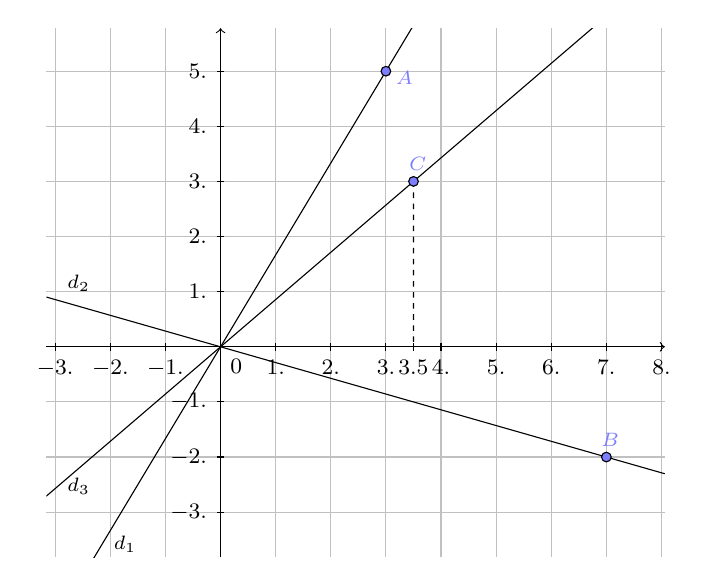
\begin{tikzpicture}[scale=0.7][line cap=round,line join=round,>=triangle 45,x=1.0cm,y=1.0cm]
\draw [color=cqcqcq,, xstep=1.0cm,ystep=1.0cm] (-3.16,-3.82) grid (8.06,5.78);
\draw[->,color=black] (-3.16,0.) -- (8.06,0.);
\foreach \x in {-3.,-2.,-1.,1.,2.,3.,3.5,4.,5.,6.,7.,8.}
\draw[shift={(\x,0)},color=black] (0pt,2pt) -- (0pt,-2pt) node[below] {\footnotesize $\x$};
\draw[->,color=black] (0.,-3.82) -- (0.,5.78);
\foreach \y in {-3.,-2.,-1.,1.,2.,3.,4.,5.}
\draw[shift={(0,\y)},color=black] (2pt,0pt) -- (-2pt,0pt) node[left] {\footnotesize $\y$};
\draw[color=black] (0pt,-10pt) node[right] {\footnotesize $0$};
\clip(-3.16,-3.82) rectangle (8.06,5.78);
\draw [domain=-3.16:8.06] plot(\x,{(-0.--1.6666666666666667*\x)/1.});
\draw [domain=-3.16:8.06] plot(\x,{(-0.-0.2857142857142857*\x)/1.});
\draw [domain=-3.16:8.06] plot(\x,{(-0.--0.8571428571428571*\x)/1.});
\draw [dash pattern=on 2pt off 2pt] (3.5010946759997243,3.000938293714049)-- (3.5005949256342954,0.);
\begin{scriptsize}
\draw[color=black] (-1.733648293963255,-3.588460111317256) node {$d_1$};
\draw[color=black] (-2.5744706911636053,1.1492022263450827) node {$d_2$};
\draw [fill=xdxdff] (3.,5.) circle (2.5pt);
\draw[color=xdxdff] (3.3370953630796135,4.871651205936921) node {$A$};
\draw [fill=xdxdff] (7.,-2.) circle (2.5pt);
\draw[color=xdxdff] (7.071443569553804,-1.6827087198515784) node {$B$};
\draw[color=black] (-2.5744706911636053,-2.5348423005565876) node {$d_3$};
\draw [fill=xdxdff] (3.5010946759997243,3.000938293714049) circle (2.5pt);
\draw[color=xdxdff] (3.5754330708661404,3.3221150278293137) node {$C$};
\end{scriptsize}
\end{tikzpicture}
\end{exercice}

\begin{exercice}
Déterminer graphiquement l'expression algébrique des fonctions affines dont les représentations graphiques sont données ci-dessous:

\definecolor{cqcqcq}{rgb}{0.752941176471,0.752941176471,0.752941176471}
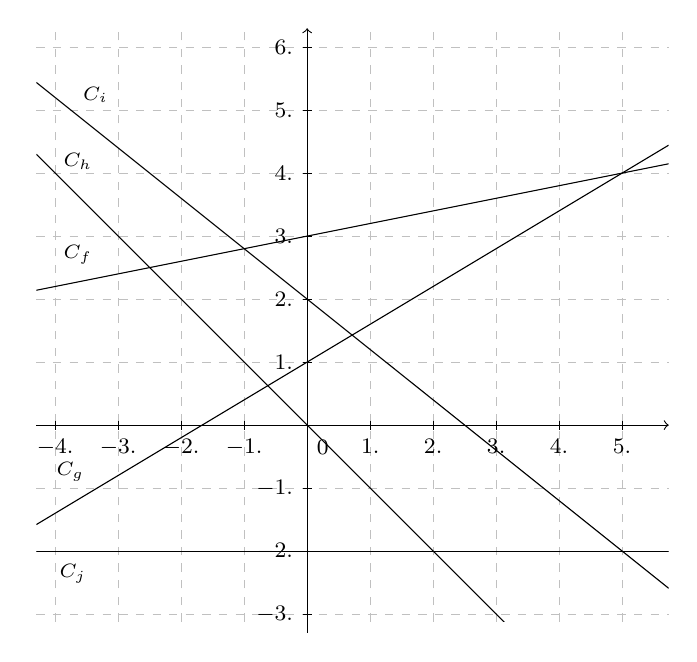
\begin{tikzpicture}[scale=0.8][line cap=round,line join=round,>=triangle 45,x=1.0cm,y=1.0cm]
\draw [color=cqcqcq,dash pattern=on 3pt off 3pt, xstep=1.0cm,ystep=1.0cm] (-4.3,-3.12) grid (5.74,6.3);
\draw[->,color=black] (-4.3,0.) -- (5.74,0.);
\foreach \x in {-4.,-3.,-2.,-1.,1.,2.,3.,4.,5.}
\draw[shift={(\x,0)},color=black] (0pt,2pt) -- (0pt,-2pt) node[below] {\footnotesize $\x$};
\draw[->,color=black] (0.,-3.3) -- (0.,6.3);
\foreach \y in {-3.,-2.,-1.,1.,2.,3.,4.,5.,6.}
\draw[shift={(0,\y)},color=black] (2pt,0pt) -- (-2pt,0pt) node[left] {\footnotesize $\y$};
\draw[color=black] (0pt,-10pt) node[right] {\footnotesize $0$};
\clip(-4.3,-3.12) rectangle (5.74,6.3);
\draw[smooth,samples=100,domain=-4.300000000000001:5.740000000000002] plot(\x,{1.0/5.0*(\x)+3.0});
\draw[smooth,samples=100,domain=-4.300000000000001:5.740000000000002] plot(\x,{3.0/5.0*(\x)+1.0});
\draw[smooth,samples=100,domain=-4.300000000000001:5.740000000000002] plot(\x,{0-(\x)});
\draw[smooth,samples=100,domain=-4.300000000000001:5.740000000000002] plot(\x,{(-4.0)/5.0*(\x)+2.0});
\draw [domain=-4.3:5.74] plot(\x,{(-2.-0.*\x)/1.});
\begin{scriptsize}
\draw[color=black] (-3.64,2.7) node {$C_f$};
\draw[color=black] (-3.76,-0.74) node {$C_g$};
\draw[color=black] (-3.64,4.18) node {$C_h$};
\draw[color=black] (-3.36,5.24) node {$C_i$};
\draw[color=black] (-3.72,-2.36) node {$C_j$};
\end{scriptsize}
\end{tikzpicture}
\end{exercice}

\begin{exercice}
Pour chacune des fonctions affines suivantes définies sur $\mathbb{R}$, précisez sa particularité (fonction linéaire, constante, identité) si elle en a une, sa pente et l'image de 0 par la fonction.\\

\begin{tabular}{p{3.5cm}p{4cm}}
\textbf{a)} $f(x)=7x-4$   &   \textbf{b)} $g(x)=x-1+1$    \\\\
\textbf{c)} $u(x)=\dfrac{-3x+1}{2}$    &  \textbf{d)} $v(x)=-3$    \\\\
\textbf{e)} $w(x)=2-x$    &  \textbf{f)} $z(x)=x^2-(x-1)^2$  
\end{tabular} 
\end{exercice}

\begin{exercice}
Déterminer la fonction affine $f$ tel que $f(1)=3$ et $f(4)=9$.
\end{exercice}

\begin{exercice}
Déterminer l'expression des fonctions affines suivantes sachant que:
\begin{enumerate}
\item $C_f$ passe par l'origine et sa pente est -1;
\item $C_g$ passe par les points $E(5;-7)$ et $F(-3;3)$;
\item $C_h$ passe par les points $A(0;3)$ et $B(5;0)$;
\item $C_i$ a pour pente -1 et l'ordonnée à l'origine de $i$ est $\dfrac{5}{8}$;
\item $C_j$ est parallèle à l'axe des abscisses et passe par le point $C(2;-3)$.
\end{enumerate}
\end{exercice}

\begin{exercice}
On considère ci-dessous les droites $d_1$ et $d_2$.
\begin{enumerate}
\item Déterminer les fonctions affines représentées par $d_1$ et $d_2$.
\item Quels sont les coordonnées exactes du point d'intersection de $d_1$ et $d_2$?
\end{enumerate}


\begin{center}
\definecolor{xdxdff}{rgb}{0.49019607843137253,0.49019607843137253,1.}
\definecolor{uuuuuu}{rgb}{0.26666666666666666,0.26666666666666666,0.26666666666666666}
\definecolor{ccqqqq}{rgb}{0.8,0.,0.}
\definecolor{qqwuqq}{rgb}{0.,0.39215686274509803,0.}
\definecolor{cqcqcq}{rgb}{0.7529411764705882,0.7529411764705882,0.7529411764705882}
\begin{tikzpicture}[line cap=round,line join=round,>=triangle 45,x=1.0cm,y=1.0cm]
\draw [color=cqcqcq,, xstep=1.0cm,ystep=1.0cm] (-3.443304347826086,-4.907513914656766) grid (4.440695652173912,5.807486085343221);
\draw[->,color=black] (-3.443304347826086,0.) -- (4.440695652173912,0.);
\foreach \x in {-3.,-2.,-1.,1.,2.,3.,4}
\draw[shift={(\x,0)},color=black] (0pt,2pt) -- (0pt,-2pt) node[below] {\footnotesize $\x$};
\draw[->,color=black] (0.,-4.907513914656766) -- (0.,5.807486085343221);
\foreach \y in {-4.,-2.,1.,2.,4.}
\draw[shift={(0,\y)},color=black] (2pt,0pt) -- (-2pt,0pt) node[left] {\footnotesize $\y$};
\draw[color=black] (0pt,-10pt) node[right] {\footnotesize $0$};
\clip(-3.443304347826086,-4.907513914656766) rectangle (9.840695652173912,5.807486085343221);
\draw[line width=1.2pt,color=qqwuqq,smooth,samples=100,domain=-3.443304347826086:9.840695652173912] plot(\x,{3.0*(\x)-2.0});
\draw[line width=1.2pt,color=ccqqqq,smooth,samples=100,domain=-3.443304347826086:9.840695652173912] plot(\x,{0-2.0*(\x)+1.0});
\begin{scriptsize}
\draw[color=qqwuqq] (-2.1191304347826083,-8.552606679035245) node {$d_1$};
\draw[color=ccqqqq] (-2.1191304347826083,5.616382189239325) node {$d_2$};
\draw [fill=uuuuuu] (0.,-2.) circle (1.5pt);
\draw[color=uuuuuu] (0.23339130434782598,-1.7001669758812623) node {$A$};
\draw [fill=xdxdff] (1.,1.) circle (2.5pt);
\draw[color=xdxdff] (1.2899130434782604,1.3574953617810728) node {$B$};
\draw [fill=uuuuuu] (0.,1.) circle (1.5pt);
\draw[color=uuuuuu] (0.14886956521739123,1.4393970315398852) node {$C$};
\draw [fill=xdxdff] (1.,-1.) circle (2.5pt);
\draw[color=xdxdff] (1.219478260869565,-0.5535435992578865) node {$D$};
\draw [fill=uuuuuu] (0.6,-0.2) circle (1.5pt);
\draw[color=uuuuuu] (0.5996521739130433,-0.7173469387755116) node {$E$};
\end{scriptsize}
\end{tikzpicture}
\end{center}
\end{exercice}

\serie{Variations}

\begin{exercice}
Déterminer le sens de variation des fonctions suivantes définies sur $\mathbb{R}$ par : 
\setlength{\columnseprule}{0pt}
\begin{multicols}{2}
\begin{enumerate}
\item $f(x)=2x+3$
\item $g(x)=-x-1$
\item $h(x)=3x+5$
\item $u(x)=-2$
\end{enumerate}
 \end{multicols}
\end{exercice}

\begin{exercice}
Déterminer le signe de $f(x)$ suivant les valeurs de $x$: 
\setlength{\columnseprule}{0pt}
\begin{multicols}{2}
\begin{enumerate}
\item $f(x)=2x+3$
\item $f(x)=-x-1$
\item $f(x)=3x+5$
\item $f(x)=-2$
\item $f(x)=-2\sqrt{2}x-1$
\end{enumerate}
 \end{multicols}
\end{exercice}

\begin{exercice}
A l'aide d'un tableau de signe, résoudre les inéquations suivantes: 
\setlength{\columnseprule}{0pt}
\begin{multicols}{2}
\begin{enumerate}
\item $-x+3>0$
\item $2x+5\leq-2$ 
\item $x^2<x^2+2x-3$
\item $-\sqrt{2}x+1\geq 0$
\end{enumerate}
 \end{multicols}
\end{exercice}

\serie{Problèmes}

\begin{exercice}
On considère un rectangle $ABDE$ et un triangle $BDC$ rectangle en $D$. On suppose que $AE=2,4$ cm, $EC=5$ cm et $CD=x$ cm.\\
\begin{enumerate}
\item Exprimer en fonction de $x$ et en $cm^2$ :
\begin{itemize}
\item l'aire $f(x)$ du triangle $BCD$
\item l'aire $g(x)$ du rectangle $ABDE$
\end{itemize}
\item Représenter graphiquement, dans un même repère, $C_f$ et $C_g$. Lire graphiquement pour quelle valeur de $x$ les deux aires sont égales.
\item Retrouver le résultat par le calcul.
\end{enumerate}
\end{exercice}

\begin{exercice}
On considère le rectangle ci-dessous.
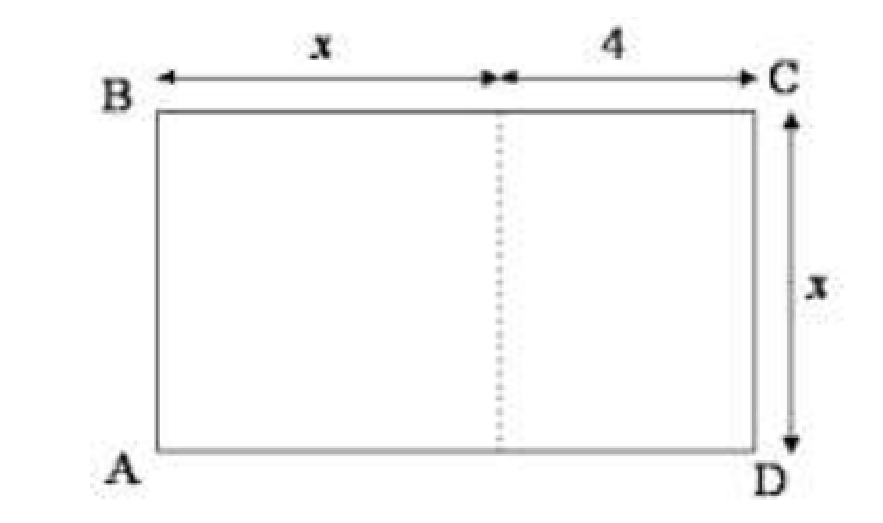
\includegraphics[scale=0.55]{FonctionsAffines/figures/FA1.eps}
Les dimensions sont exprimées en cm.
$x$ désigne un nombre strictement positif.
\begin{enumerate}
\item Écrire, en fonction  de $x$, le périmètre de ABCD que l’on notera $P(x)$. 
Montrer que $P$ est une fonction affine.
\item Déterminer le périmètre du rectangle ABCD lorsque $x=3,2$.
\item  Quelle doit être la valeur de$x$   afin que le périmètre de ce rectangle soit de 26 cm ?
\item
\begin{enumerate}
\item Exprimer, en fonction de $x$, l’aire de ce rectangle qu’on notera $A(x)$.
\item La fonction $A$  est-elle une fonction affine ? Justifier.
\end{enumerate}
\end{enumerate}
\end{exercice}

\begin{exercice}
Deux chauffeurs de taxi pratiquent des tarifs différents :
\begin{itemize}
\item Tarif A : 5 euros de prise en charge et 0,40 euros par km parcouru
\item Tarif B : pas de frais de prise en charge mais 0,60 euros par kilomètre parcouru. 
\end{itemize}
\begin{enumerate}
\item Exprimer $A(x)$ le prix payé au taxi $A$ et $B(x)$ le prix payé au taxi $B$ en fonction du nombre de kilomètres parcourus $x$
\item Représenter graphiquement les deux fonctions $A$ et $B$
\item Déterminer graphiquement pour quelles longueurs de trajet vaut-il mieux prendre le taxi $A$?
\item Retrouver le résultat par un calcul.
\end{enumerate}
\end{exercice}


\begin{exercice}
Un club édite un magazine de "Jeunesse" qui paraît chaque lundi. Il propose deux tarifs :
\begin{itemize}
\item tarif 1 : pour les non-adhérents, 2CHF par magazine acheté;
\item tarif 2 : pour les adhérents, une cotisation annuelle de 20 CHF, chaque magazine est alors payé 1,2 CHF.
\end{itemize}
\begin{enumerate}
\item Pour chacun des tarifs, calculer le prix payé pour 10, 20, 30, 50 magazines.
\item Jean apprécie ce magazine et l'achète quelquefois.

On appelle $x$ le nombre de magazines "Jeunesse" que Jean achète dans une année.

On appelle $f(x)$ le prix à payer avec le tarif 1 et $g$ le prix à payer avec le tarif 2.

Déterminer $f(x)$
\item Représenter dans le même repère les fonction $f$ et $g$
\item Utiliser un graphique pour trouver pour quel valeur de $x$ les deux tarifs mènent à la même dépense
\item Retrouver le résultat par un calcul.
\end{enumerate}
\end{exercice}

\begin{exercice}
Soit $ABC$ un triangle rectangle en $A$ tel que $AB=6$ cm et $AC=8$ cm.\\ Soit $M\in[AB]$ (distinct de $A$ et de $B$), la parallèle à $(BC)$ passant par $M$ coupe $[AC]$ en $N$. On pose $BM=x$.

Trouvez l'ensemble des valeurs de $x$ pour lesquelles le périmètre du triangle $AMN$ est inférieur ou égale au périmètre du trapèze $MNCB$. Justifiez graphiquement votre réponse. Précisez toutes les étapes de votre recherche.
\end{exercice}

\begin{exercice}
Un promeneur marche pendant deux heures à la vitesse moyenne de 6 $km/h$, s'arrête 30 minutes, puis rentre chez lui à la bicyclette par le même chemin. La situation est représentée sur la figure suivante.
 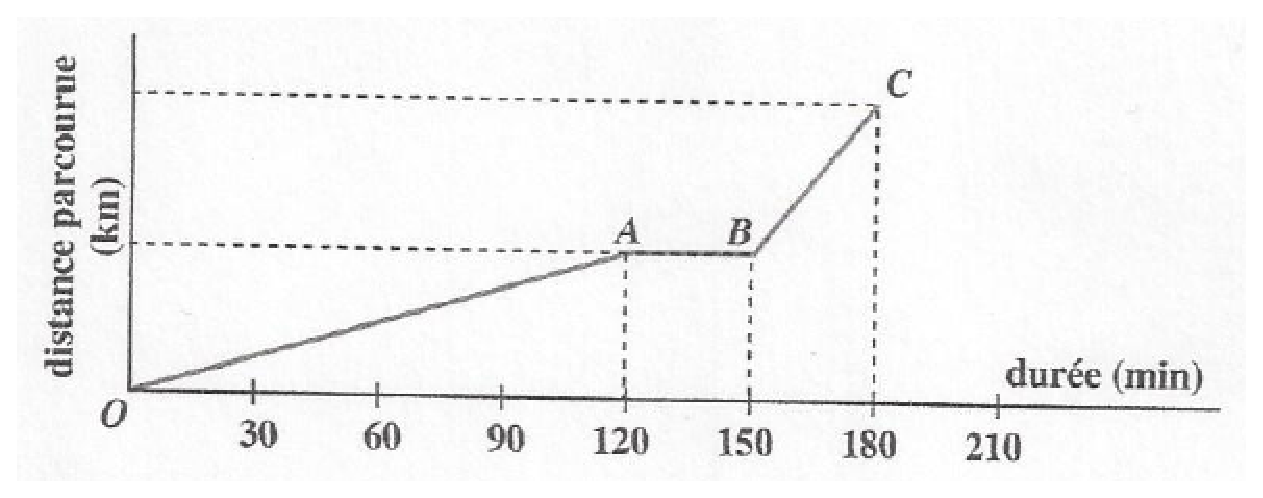
\includegraphics[scale=0.4]{FonctionsAffines/figures/FA2.eps}
\begin{enumerate}
\item Déterminer les trois fonctions affines dont les représentations graphiques contiennent respectivement $O$ et $A$,  $A$ et $B$, $B$ et $C$.
\item En déduire la distance parcourue au bout de 80 minutes et de 160 minutes.
\end{enumerate}
\end{exercice}
\end{colonne*exercice}

\connaissances
%\begin{acquis}
\begin{itemize}
\item BlaBla1
\item BlaBla2
\item BlaBla3
\item BlaBla4
\item BlaBla5
\item BlaBla6
\end{itemize}
\end{acquis}

\QCMautoevaluation{Pour chaque question, plusieurs réponses sont
  proposées.  Déterminer celles qui sont correctes.} % Est-ce que c'est toujours le cas ?

\begin{QCM}
  \begin{GroupeQCM} % Est-ce qu'on les séparent en groupe ?
    \begin{exercice}
      Quelle est la bonne réponse ?
      \begin{ChoixQCM}{4}
      \item un
      \item deux
      \item trois
      \end{ChoixQCM}
\begin{corrige}
     \reponseQCM{ab} % ici deux réponses justes
   \end{corrige}
    \end{exercice}


\end{GroupeQCM}
\end{QCM}

  

\pagebreak



